\documentclass{beamer}

%% FORMATTING
% ----------------------------------------------------------------------------- %
%\usepackage[margin=1in]{geometry} % margins
%\usepackage[doublespacing]{setspace} % line spacing
\usepackage{xcolor, cite}
\usepackage{
    multicol, % multiple columns
    blindtext, % \blindtext (lorem ipsum)
    lipsum,
    tikz,
    graphicx,
    booktabs,
    amsmath,
    amssymb,
    hyperref,
    graphicx,
    makecell,
    array,
    subcaption,
    adjustbox,
    etoolbox
}

\usepackage{wrapfig}
\usepackage{parskip} % distance between paragraphs; care with theorem environment
\usepackage{algorithm2e}
\usepackage{algorithmic}
\setlength{\parskip}{0.5cm plus4mm minus3mm}
\usetheme{Madrid}

%\usecolortheme{crane}

\definecolor{MasonGreen}{RGB}{30, 98, 56}
\definecolor{MasonGold}{RGB}{226, 168, 43}

\setbeamercolor{palette primary}{bg=MasonGreen, fg=MasonGold}
\setbeamercolor{palette secondary}{bg=MasonGreen, fg = MasonGreen}
\setbeamercolor{palette tertiary}{bg=MasonGold, fg = MasonGreen}
\setbeamercolor{palette quaternary}{bg=MasonGold, fg = MasonGreen}
\setbeamertemplate{bibliography item}{\insertbiblabel}

\newcolumntype{M}[1]{>{\centering\arraybackslash}m{#1}}


\graphicspath{{./figures/}}
% graphics should go into the ./figures/ folder
\blindmathtrue


%% MATH %%
% ----------------------------------------------------------------------------- %
\usepackage{ 
    mathtools, % advanced math (superset of amsmath)
    % thmtools,
    amssymb, % additional math symbols
    amsthm, % proof environment and \theoremstyle
    mathrsfs, % scripty math
    % stmaryrd % contains \lightning
}

%% OPERATORS / DELIMITERS
% ----------------------------------------------------------------------------- %
% \operatorname{Example} for single use
% \DeclareMathOperator{\example}{Example}
\DeclarePairedDelimiter{\abs}{\lvert}{\rvert}
\DeclareMathOperator{\injects}{\hookrightarrow}
\DeclareMathOperator{\iso}{\cong}
\DeclareMathOperator{\Aut}{Aut}
\DeclareMathOperator{\Orb}{Orb}

%% REFERENCE
% ----------------------------------------------------------------------------- %
\usepackage{ 
    % nameref, % \nameref
    % hyperref % hyperlink/reference
}

\title{Work unit evolution: Using large language models to determine temporal task evolution}
\author{Bryan Adams}
\institute{George Mason University}
\date{\today}



\begin{document}

\begin{frame}
  \titlepage
\end{frame}

\begin{frame}
  \frametitle{Table of Contents}
  % \addtolength{\leftskip}{-2em} % Adjust the left indentation
  % \addtolength{\rightskip}{-2em} % Adjust the right indentation
  \tableofcontents
\end{frame}

% ----------------------------------------------------------------------------- %
\section{Motivation}

\begin{frame}{Motivation}
  \begin{itemize}
    \item Identifying relevant knowledge, skills, and abilities (KSAs) has been extensively researched in economics, management and sociology. \cite{investment_human_capital, task_specific, on_the_mechanics, diversification}
    \item Classifying KSAs is also extensively researched in many fields. \cite{specialization_career,industry-specific_human_capital, human_capital_specificity}
    \item The majority of previous research focused on unifying KSAs into one taxonomy as "tasks" and relied on survey data which forces participants to bin their occupational requirements.\cite{nested_skills, how_general_is_human_capital} 
    \item Previous research focused on industry or country level aggregation of occupational requirements.
    \item With the advancement of large language models (LLMs), could we identify occupational requirements for a specific position and how they evolve over time? 
  \end{itemize}
\end{frame}

% ----------------------------------------------------------------------------- %
\section{USAJobs job ads}

\begin{frame}{USAJobs job ads}
  Analyzing job ads for the Army Acquisitions Workforce (AAW)

  \vspace{.25cm}

  In September 2023, USAJobs\footnote{Job ads were pulled from \href{https://developer.USAJobs.gov/API-Reference/}{https://developer.USAJobs.gov/API-Reference/}} contained \textbf{2,379,956 }of historical job ads with position opening dates from 2012-09-12 to 2027-05-26. The following filtering criteria were applied to determine the relevant AAW job ads. The filtering resulted in a possible \textbf{75,914} job ads related to AAW with position opening dates from 2015-02-01 to 2023-10-22.

  \begin{enumerate}
    \item Filter on job ads with a hiring department of \textit{Department of the Army} or \textit{Department of the Defense} reducing the number of job ads to \textbf{772,297}.
    \item Search job add for the term \textit{acquisition} reducing the number of job ads to \textbf{79,071}.
  \end{enumerate}

\end{frame}

% ----------------------------------------------------------------------------- %

\begin{frame}{USAJobs job ads}
  \small
  \vspace*{-1.1cm}
  \begin{table}[ht!]
    \centering
    \vspace*{4mm}
    \begin{subtable}[t]{0.4\linewidth}
        \centering
        \caption{Historical job posting counts by position opening year}
        % \begin{adjustbox}{valign=t}
        \begin{tabular}{cc}
            \Xhline{3\arrayrulewidth}
            Year &   Count \\\Xhline{3\arrayrulewidth}
            2012 &       1 \\
            2013 &       6 \\
            2014 &      23 \\
            2015 &     143 \\
            2016 &    3893 \\
            2017 &  237451 \\
            2018 &  329440 \\
            2019 &  348783 \\
            2020 &  328452 \\
            2021 &  369111 \\
            2022 &  441709 \\
            2023 &  320874 \\
            2024 &      69 \\
            2027 &       1 \\
            \Xhline{3\arrayrulewidth}
        \end{tabular}\label{tab:job_opening_count}
    % \end{adjustbox}
    \end{subtable}
    \begin{subtable}[t]{0.4\linewidth}
        \centering
        \caption{Possible AAW historical job posting counts by position opening year}
        % \begin{adjustbox}{valign=t}
        \vspace*{4mm}
        \begin{tabular}{cc}
            \Xhline{3\arrayrulewidth}
                Year &  Count\\\Xhline{3\arrayrulewidth}
                2015 &      5\\
                2016 &     39\\
                2017 &   7537\\
                2018 &  12033\\
                2019 &  13087\\
                2020 &  10320\\
                2021 &  11619\\
                2022 &  12567\\
                2023 &   8707\\
            \Xhline{3\arrayrulewidth}
        \end{tabular}\label{tab:aaw_job_opening_count}
        % \end{adjustbox}
    \end{subtable}
\end{table}
  
\end{frame}

% ----------------------------------------------------------------------------- %

\begin{frame}{USAJobs job ad example}
  \scriptsize
  \begin{exampleblock}{Raw job ad}
    To qualify for a Contract Specialist your resume and supporting documentation must support: $<$br /$>$\textbackslash n$<$br /$>$\textbackslash nA. . Basic DoD 1102 Requirement: Public Law 106-398, Section 808: A.) A baccalaureate degree from an accredited educational institution authorized to grant baccalaureate degrees AND B.) at least 24 semester hours (or equivalent) of study from an ... Creditable specialized experience includes:$<$br /$>$\textbackslash n$<$br /$>$\textbackslash nGS-13:\textbackslash n$<$ul$>$\textbackslash n \textbackslash t$<$li$>$Developing contractual strategies.$<$/li$>$\textbackslash n \textbackslash t$<$li$>$Ensuring acquisition plans are in full compliance with contracting regulations and related Department of Defense (DoD) standards.$<$/li$>$\textbackslash n \textbackslash t$<$li$>$Planning and conducting negotiations on price, technical requirements, terms, and conditions of the contract.$<$/li$>$\textbackslash n \textbackslash t$<$li$>$Developing acquisitions strategies and/or determining methods of procurement and ensuring proper performance.$<$/li$>$\textbackslash n$<$/ul$>$\textbackslash nGS-12:\textbackslash n\textbackslash n$<$ul$>$\textbackslash n \textbackslash t$<$li$>$Verifies for accuracy purchase requests, prepares acquisition plans, conducts market research and recommends contract type and pricing strategies.$<$/li$>$\textbackslash n \textbackslash t$<$li$>$Performs price and cost analysis, analyzing unit costs and pricing data and contractors projected costs.$<$/li$>$\textbackslash n \textbackslash t$<$li$>$Performs full range of contract administration functions.$<$/li$>$\textbackslash n \textbackslash t$<$li$>$Assists with extensive negotiations which address acquisition related issues with offerors.$<$/li$>$\textbackslash n \textbackslash t$<$li$>$Assists to prepare and issue contract modifications under long term contracts.$<$/li$>$\textbackslash n \textbackslash t$<$li$>$Assists in developing contractual strategies.$<$/li$>$\textbackslash n \textbackslash t$<$li$>$Develops cost and price analysis spreadsheets for long-term contracts.$<$/li$>$\textbackslash n$<$/ul$>$\textbackslash nE...      
  \end{exampleblock}
\end{frame}

% ----------------------------------------------------------------------------- %

\begin{frame}{USAJobs job ad example}
  Removed html tags, common phrases and unnecessary characters.
  \scriptsize
  \begin{exampleblock}{Cleaned job ad}
    To qualify for a Contract Specialist your resume and supporting documentation must support:A. Basic DoD 1102 Requirement: Public Law 106-398, Section 808: A.) A baccalaureate degree from an accredited educational institution authorized to grant baccalaureate degrees AND B.) at least 24 semester hours (or equivalent) of study from an ... Creditable specialized experience includes:GS-13:Developing contractual strategies.Ensuring acquisition plans are in full compliance with contracting regulations and related Department of Defense (DoD) standards.Planning and conducting negotiations on price, technical requirements, terms, and conditions of the contract.Developing acquisitions strategies and/or determining methods of procurement and ensuring proper performance.GS-12:Verifies for accuracy purchase requests, prepares acquisition plans, conducts market research and recommends contract type and pricing strategies.Performs price and cost analysis, analyzing unit costs and pricing data and contractors projected costs.Performs full range of contract administration functions.Assists with extensive negotiations which address acquisition related issues with offerors.Assists to prepare and issue contract modifications under long term contracts.Assists in developing contractual strategies.Develops cost and price analysis spreadsheets for long-term contracts.
  \end{exampleblock}
\end{frame}

% ----------------------------------------------------------------------------- %
\section{Knowledge, skills and abilities (KSAs)}
% \subsection{Occupational Information Network (O\textsuperscript{*}NET)}

\begin{frame}{Occupational Information Network (O\textsuperscript{*}NET)}

  O\textsuperscript{*}NET created and currently maintains occupation specific descriptors. These descriptors created the O\textsuperscript{*}NET content model, which is used to define occupations within Standard Occupational Classification (SOC) system.\footnote{Data files available at \href{https://www.onetcenter.org/content.html}{https://www.onetcenter.org/content.html}}
  \begin{columns}
    \begin{column}{0.4\textwidth}
      \begin{itemize}
        \item \textbf{33 knowledges}\cite{knowledges}
        \item \textbf{46 skills}\cite{skills}
        \item \textbf{52 abilities}\cite{abilities}
        \item 42 generalized work activities
        \item 46 aspects of work context
        \item 21 occupational values
        \item 17 work style requirements
      \end{itemize}
    \end{column}
    \begin{column}{0.6\textwidth}
      \begin{figure}[ht!]
        \centering
        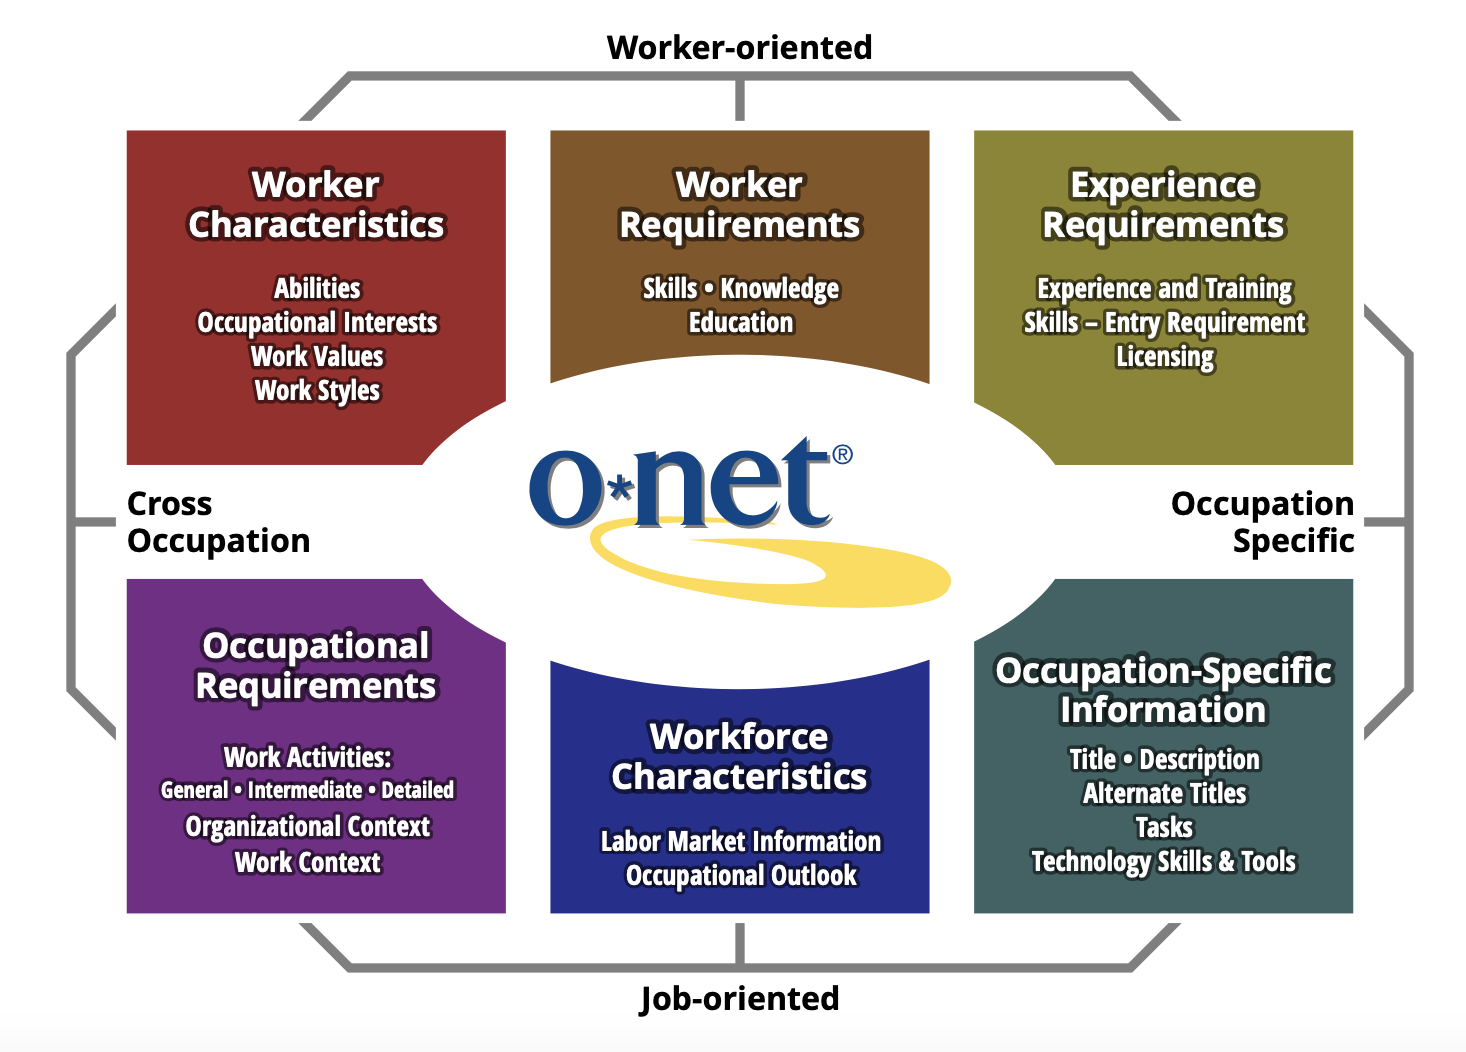
\includegraphics[width=0.95\textwidth]{images/onet.png}
      \end{figure}
    \end{column}
  \end{columns}
\end{frame}

% ----------------------------------------------------------------------------- %
\begin{frame}{Example O\textsuperscript{*}NET knowledge definitions\footnote{Data files available at \href{https://www.onetcenter.org/database.html\#individual-files}{https://www.onetcenter.org/database}}}
  \small
  \begin{itemize}
    \item Administration and Management - Knowledge of business and management principles involved in strategic planning, resource allocation, human resources modeling, leadership technique, production methods, and coordination of people and resources.
    \item Administrative - Knowledge of administrative and office procedures and systems such as word processing, managing files and records, stenography and transcription, designing forms, and workplace terminology.
    \item Mathematics - Knowledge of arithmetic, algebra, geometry, calculus, statistics, and their applications.
    \item Engineering and Technology - Knowledge of the practical application of engineering science and technology. This includes applying principles, techniques, procedures, and equipment to the design and production of various goods and services.
  \end{itemize}  
\end{frame}

% ----------------------------------------------------------------------------- %
\section{Identifying KSAs in job ads using using Pathways Language Model (PaLM)}
\begin{frame}{PaLM - Pathways Language Model\cite{palm}}
  \begin{itemize}
  \item PaLM uses a standard Transformer model architecture similar to the architecture described in \textit{Attention is all you need}. 

  \item The significant changes are:

  \begin{itemize}
    \item Uses SwiGLU activation function
    \item Parallel Layers in each Transformer block
    \item Transformer formulation uses $k$ attention heads
    \item RoPE embeddings instead of absolute or relative position embeddings 
    \item Use SentencePiece for vocabulary
  \end{itemize}

  \item 540 billion parameters, 118 layers, and 48 attention heads

  \item PaLM2 is an update on PaLM but trained on a larger more diverse data set and redesigned for more compute efficiency.\cite{palm2}

  \end{itemize}
\end{frame}

% ----------------------------------------------------------------------------- %

\begin{frame}{SwiGLU activation function\cite{swiglu}}
  \scriptsize

  SwiGLU activation function combines the Swish activation function\cite{swish} and gated linear units (GLU)\cite{glu}.

  \begin{columns}
    \begin{column}{0.55\textwidth}
      \begin{itemize}
        \item Swish activation function
        \begin{itemize}
          \item $Swish(x) = x\sigma(\beta x), \sigma(z) = (1+e^{-z})^{-1}$
          \item Improvement over ReLU $=max(0,x)$
        \end{itemize}
        \item GLU
        \begin{itemize}
          \item $h_l(\mathbf{X}) = (\mathbf{X} * \mathbf{W}+ b) \otimes (\mathbf{X} * \mathbf{V} + c)$
          \begin{itemize}
            \item $h_l = $ hidden layer
            \item $\mathbf{X} = $ input layer
            \item $\mathbf{V} = $ words in model vocabulary
            \item $\mathbf{W} = $ learned parameters
          \end{itemize}
        \end{itemize}
        \item SwiGLU
        \begin{itemize}
          \item $Swish_{\beta}(x\mathbf{W}+ b) \otimes (x\mathbf{V} + c)$
          \item PaLM uses $Swish_{\beta}(x \mathbf{W}) \otimes (x \mathbf{V})$
        \end{itemize}
      \end{itemize}
    \end{column}
    \begin{column}{0.5\textwidth}
      \begin{figure}[ht!]
        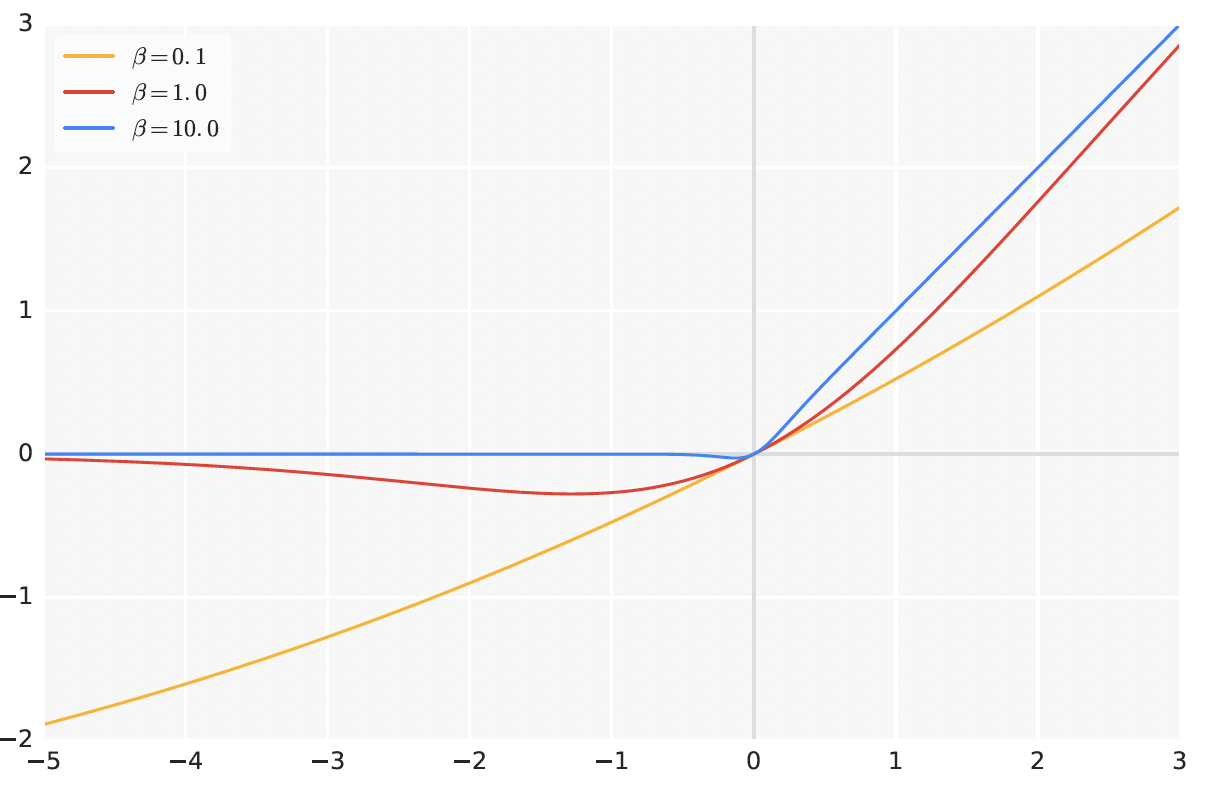
\includegraphics[width=0.6\textwidth]{images/swish_act.png}
        \caption{Swish activation function\cite{swish}}
      \end{figure}
    \end{column}
  \end{columns}
  
\end{frame}

% ----------------------------------------------------------------------------- %
% \section{Identifying KSAs in job ads using}

\begin{frame}{Identifing KSAs in job ads}

  The following is the prompt structure provide to PaLM2 to extract KSAs from a specific job ad.

  \begin{exampleblock}{Leading text provided to PaLM2}
    $<$knowledge name$>$ is the $<$knowledge description$>$. Look at the job ad and decide if $<$knowledge name$>$ is required to perform this job. If $<$knowledge name$>$ is required please provide the specific tasks in a bulletized format from the job ad that relate to $<$knowledge name$>$, if not simply say no.
  \end{exampleblock}
  \begin{exampleblock}{Query provided to PaLM2}
    Does this job ad require $<$knowledge name$>$ knowledge to perform the job?
  \end{exampleblock}
  
\end{frame}

% ----------------------------------------------------------------------------- %

\begin{frame}{Example PaLM2 response for Administration and Management}
  \scriptsize
  Candidate 1: Yes.

  The job ad requires the following skills:

  \begin{itemize}
    \item Knowledge of Federal and agency contracting laws and regulations applicable to centralized acquisition of agency-wide commodity and service requirements
    \item Knowledge of commercial business and industry practices and trends, cost factors, and market conditions along with understanding the military support requirements to be procured to identify potential contractors in limited supplier source situations.
    \item Developing of pre-negotiation plans, negotiation techniques, and cost and price analysis of procurement proposals to independently decide on proper strategies to procure complex requirements.
    \item Applying negotiation, persuasion and compromise techniques is required to negotiate price, terms and conditions, delivery schedule, contract modifications, (quantity options and extension of contract performance periods) and settlement of contractor claims in the best interest of the Government.
  \end{itemize}
  
\end{frame}

% ----------------------------------------------------------------------------- %

\begin{frame}{Identifing KSAs in job ads}

\begin{itemize}
  \item Temperature [0,1] = 0.5 - Controls the randomness of the output, higher values produce more varied responses
  \item Retrieve \textbf{3} candidate answers and if all are \textbf{yes} the KSA is added to the job KSA vector
\end{itemize}

\begin{exampleblock}{Example KSA vector}
  [Physics, Mathematics and Science, Economics and Accounting, Business and Management, Education and Training, Mathematics, Chemistry, Engineering and Technology]
\end{exampleblock}
  
\end{frame}

% ----------------------------------------------------------------------------- %

\section{Defining the KSA vector space using Bidirectional Encoder Representations from Transformers (BERT) and Sentence-BERT (SBERT)}

\begin{frame}{How close are two job requirements?}

  We need to define a vector space to measure how job requirements evolve overtime. In this figure, the job KSAs changed between $t$ and $t+m$ as well as $t+m$ and $t+n$.

  \begin{columns}
    \begin{column}{0.5\textwidth}
      \textbf{Example job KSA vectors}
      \vspace{.25cm}
      \begin{itemize}
        \item $t$ = [Engineering and Technology, Mathematics]
        \item $t+m$ = [Engineering and Technology, Physics]
        \item $t+n$ = [Business and Management, Economics and Accounting]
      \end{itemize}
      
    \end{column}
    \begin{column}{0.5\textwidth}
      \begin{figure}[ht!]
        \centering
        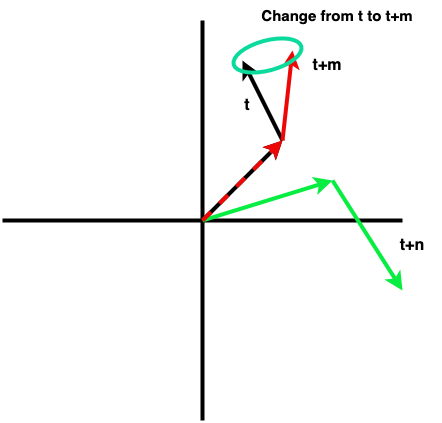
\includegraphics[width=0.6\textwidth]{images/task_change_w_time.png}
        \caption{Representation of job KSA vector changes}
      \end{figure}\label{fig:change}
    \end{column}
  \end{columns}
\end{frame}

% ----------------------------------------------------------------------------- %

% \subsection{BERT - Bidirectional Encoder Representations from Transformers}

\begin{frame}{Creating vector space for KSAs using BERT}

  BERT - Bidirectional Encoder Representations from Transformers\cite{bert}
  \begin{itemize}
    \item Multi-layer bidirectional Transformer encoder based on \textit{Attention Is All You Need}.\cite{attention}
    \item BERT\textsubscript{BASE} - 12 layers, hidden size is 768, 12 attention heads, 110 million parameters
    \item Minimized cross entropy loss
  \end{itemize}
  
  \begin{figure}[ht!]
    \centering
    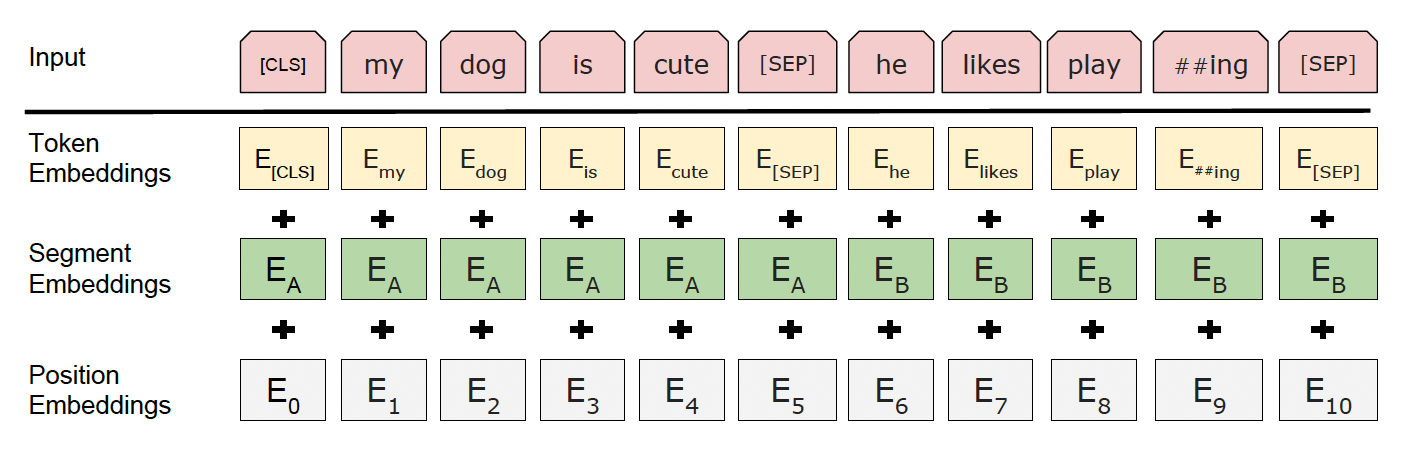
\includegraphics[width=0.9\textwidth]{images/bert.png}
  \end{figure}
  
\end{frame}

% ----------------------------------------------------------------------------- %

\begin{frame}{Tuning BERT model}
 \scriptsize
  Used batch size of \textbf{16}, \textbf{2} epochs and masked \textbf{15\%} of the tokens

  \begin{exampleblock}{Tokenized knowledge description}
    ['[CLS]','principles','and','facts','related','to','business','administration',
    'and','accounting',',','human','and','material','resource','management','in',
    'organizations',',','sales','and','marketing',',','economics',',','and',
    'office','information','and','organizing','systems','[SEP]','[PAD]',...]
  \end{exampleblock}

  \begin{exampleblock}{Whole word masking}
    ['[CLS]','[MASK]','and','[MASK]','related','to','business','[MASK]',
    'and','accounting',',','human','and','[MASK]','resource','management',
    'in','organizations',',','sales','and','marketing','[MASK]','economics',
    '[MASK]','and','office','information','and','organizing','systems',
    '[SEP]','[PAD]'...]
  \end{exampleblock}

  \begin{exampleblock}{Wordpiece\cite{wordpiece} tokenizing}
    [['[CLS]','principle','\#\#s','and','facts','related','to','business','administration',
    'and','accounting',',','human','and','material','resource','management','in',
    'organizations',',','sales','and','marketing',',','economics',',','and',
    'office','information','and','organizing','systems','[SEP]']]
  \end{exampleblock}
  
\end{frame}

% ----------------------------------------------------------------------------- %

\begin{frame}{Tuning BERT model}
  Used \textbf{Adam} instead of \textbf{stochastic gradient descent}. \textbf{Adam} is a method for efficient stochastic optimization that only requires first-order gradients with little memory requirement.\cite{kingma2017adam}
  \begin{columns}
    \begin{column}{0.3\textwidth}
      \begin{itemize}
        \item Learning rate (step size): $\alpha = 0.00005$
        \item Hyper-parameters for decay rates of moving averages: $\beta_1 = 0.9$, $\beta_2 = 0.98$
        \item Correct initialization bias
      \end{itemize}
    \end{column}
    \begin{column}{0.7\textwidth}
        \begin{figure}[ht!]
          \centering
          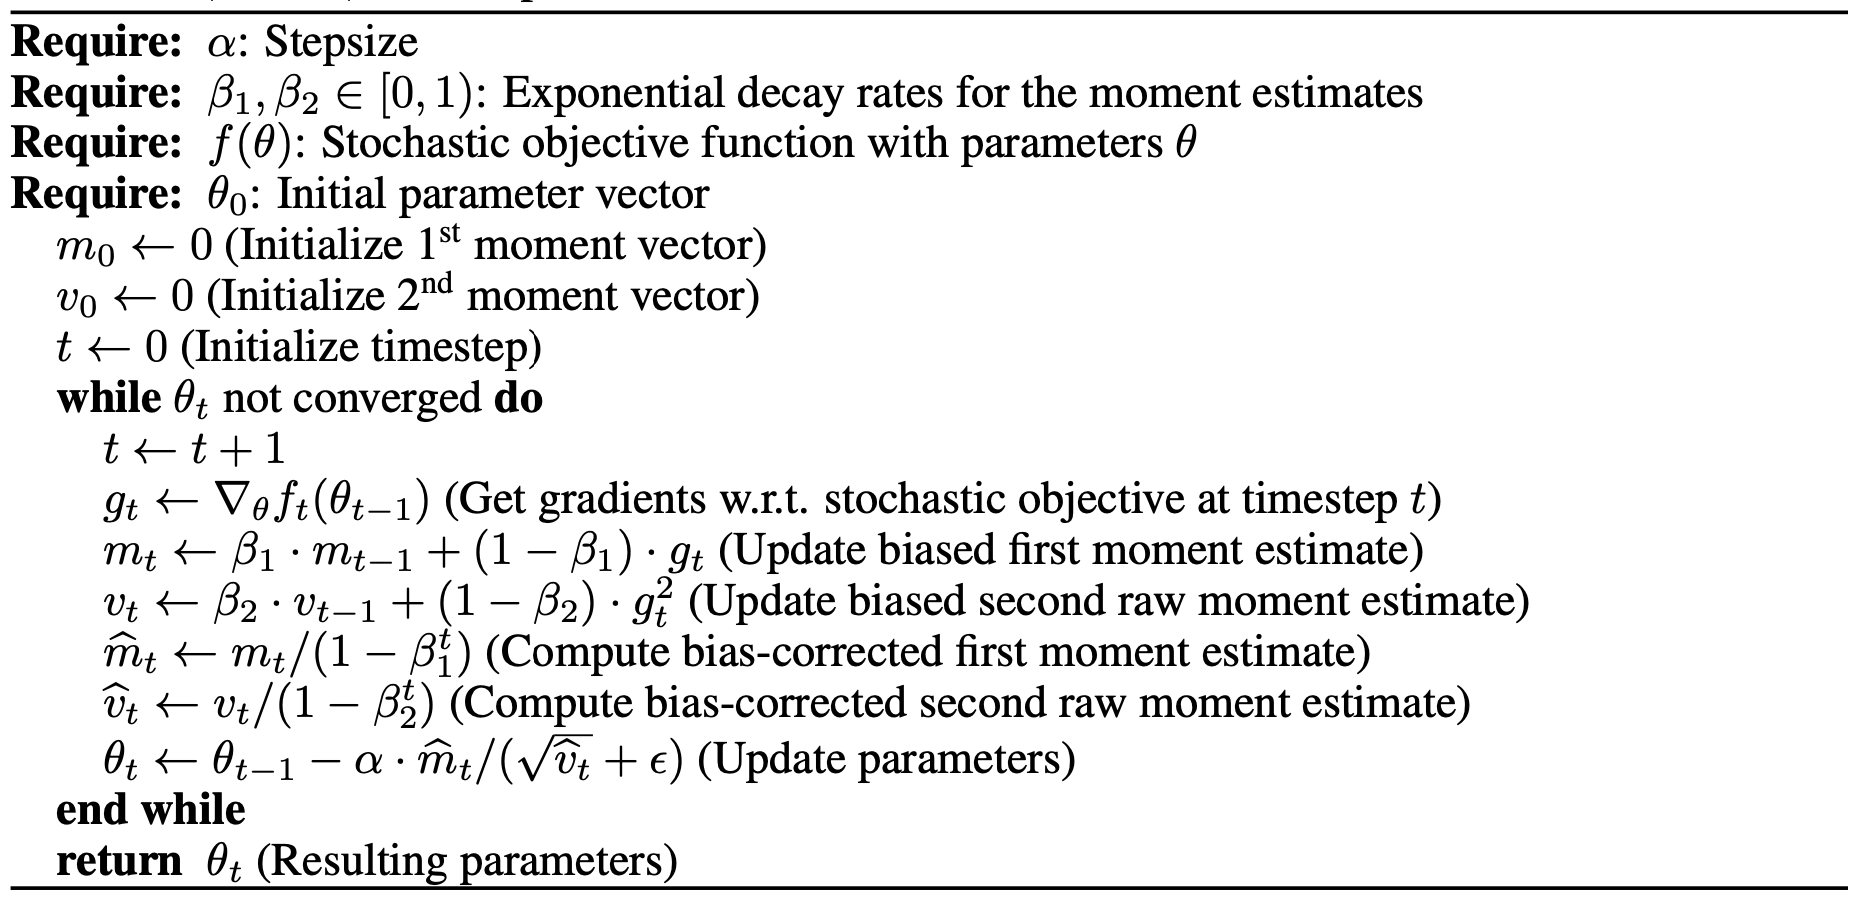
\includegraphics[width=0.9\textwidth]{images/adam_opt.png}
      \end{figure}     
    \end{column}
  \end{columns}
\end{frame}

% ----------------------------------------------------------------------------- %

% \subsection{Sentence-BERT (SBERT)}

\begin{frame}{Sentence-BERT (SBERT)\cite{sbert}}
  The objective is to determine which sentence pairs are similar (should be close in vector space) and which pairs are dissimilar (should be far away in vector space)
  \begin{columns}
    \begin{column}{0.4\textwidth}
     \begin{itemize}
      \item SBERT adds a pooling operation to the output of BERT
      \item Mean pools the BERT hidden layers
      \item Computes the cosine similarity between the two embeddings: $\frac{\vec{u} \cdot \vec{v}}{\|\vec{u}\|\|\vec{v}\|}$
     \end{itemize}
    \end{column}
    \begin{column}{0.6\textwidth}
        \begin{figure}[ht!]
          \centering
          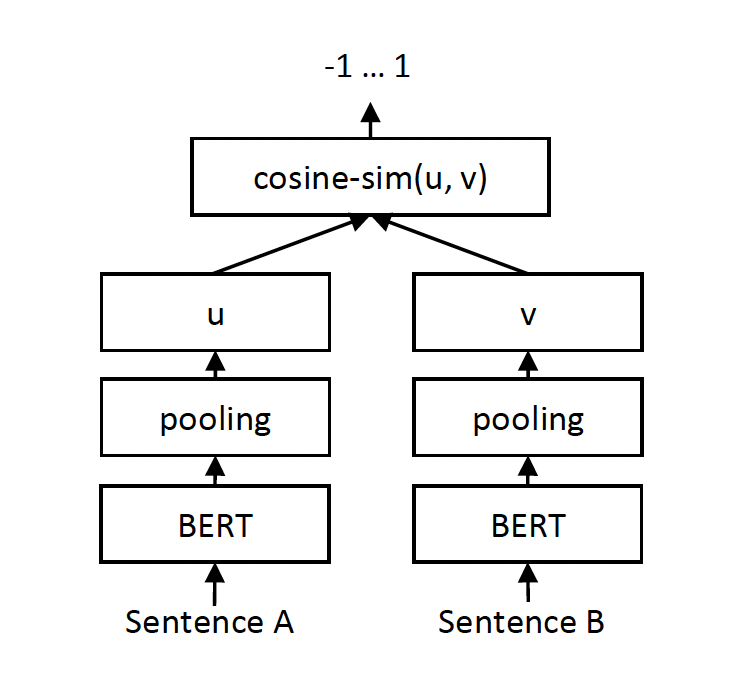
\includegraphics[width=0.9\textwidth]{images/sbert_arch.png}
      \end{figure}     
    \end{column}
  \end{columns}
\end{frame}

% ----------------------------------------------------------------------------- %

\section{Comparison of methods}

\begin{frame}{SBERT vector embeddings projection}
  \begin{figure}[ht!]
    \centering
    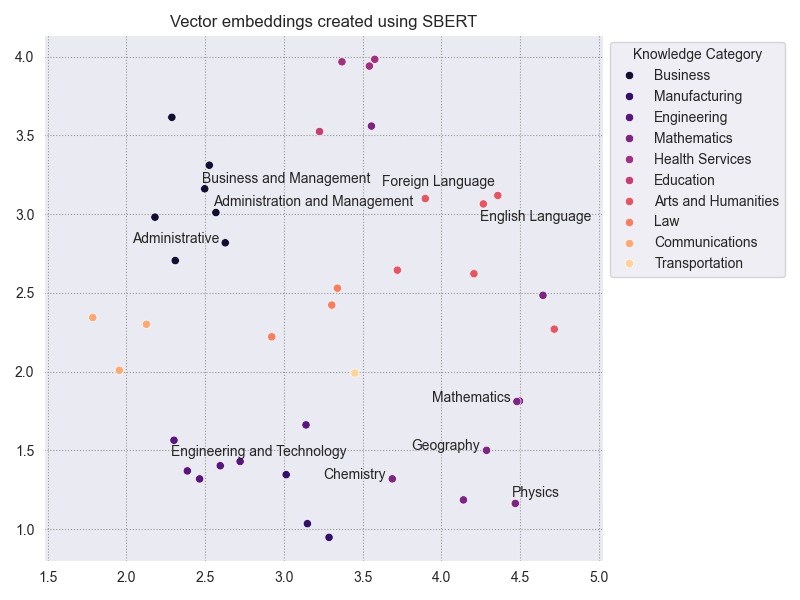
\includegraphics[width=0.9\textwidth]{../plots/base_sbert.png}
\end{figure}

\end{frame}

% ----------------------------------------------------------------------------- %

\begin{frame}{Tuned BERT vector embeddings projection}
  \begin{figure}[ht!]
    \centering
    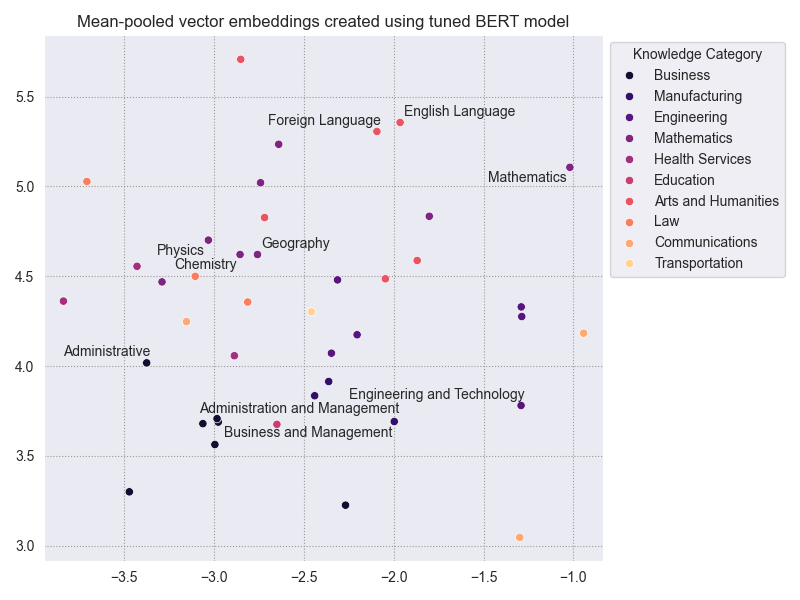
\includegraphics[width=0.9\textwidth]{../plots/tuned_bert.png}
\end{figure}

\end{frame}

% ----------------------------------------------------------------------------- %

\begin{frame}{BERT vector embeddings projection}
  \begin{figure}[ht!]
    \centering
    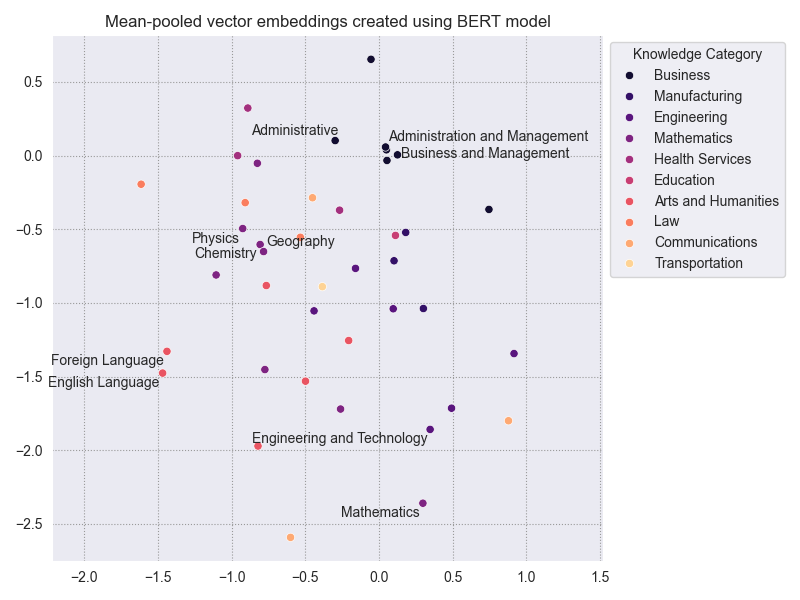
\includegraphics[width=0.9\textwidth]{../plots/base_bert.png}
\end{figure}

\end{frame}

% ----------------------------------------------------------------------------- %

\begin{frame}{Comparison of model results}

  \begin{table}[h!]
    \centering
    \caption{Cosine similarity between knowledge descriptions}
    \vspace*{-6mm}
    \begin{tabular}{m{3cm}m{3cm}M{1cm}M{1cm}M{1cm}}
      \Xhline{3\arrayrulewidth}
      \multicolumn{1}{m{3cm}}{\centering \textbf{Element 1}}& 
      \multicolumn{1}{m{3cm}}{\centering \textbf{Element 2}} & 
      \multicolumn{1}{m{1cm}}{\centering \textbf{SBERT}} & 
      \multicolumn{1}{m{1cm}}{\centering \textbf{Tuned BERT}} & 
      \multicolumn{1}{m{1cm}}{\centering \textbf{BERT base}} \\\Xhline{3\arrayrulewidth}
      Business and Management & Administration and Management & 0.731 & 0.859 & 0.865 \\\hline
      Administration and Management & Administrative & 0.336 & 0.759 & 0.782 \\\hline
      Mathematics & Physics & 0.264 & 0.719 & 0.742 \\\hline
      Engineering and Technology & Mathematics & 0.277 & 0.727 & 0.732 \\\hline
      Administrative & Mathematics & 0.203 & 0.702 & 0.722 \\\hline
      English Language & Foreign Language & 0.831 & 0.941 & 0.965 \\\hline
      Mathematics & English Language & 0.170 & 0.706 & 0.724 \\
      \Xhline{3\arrayrulewidth}
      \end{tabular}
  \end{table}
  
\end{frame}

% ----------------------------------------------------------------------------- %
\section{Future work}

\begin{frame}{Future work}
  \begin{itemize}
    \item PaLM2 prompt generation - providing more specificity in prompt will increase validity of response, e.g. add examples of misclassification to the prompt
    \item Determine the optimal model to use to define the vector space of KSAs
  \end{itemize}
  
\end{frame} 

% ----------------------------------------------------------------------------- %
\section{References}

\begin{frame}[allowframebreaks]
  \frametitle{References}
  \tiny
  \bibliographystyle{siam}
  \bibliography{refs}
\end{frame}

% \begin{frame}{Bib}
%   \bibliographystyle{plain}
%   \bibliography{refs}
% \end{frame}


\end{document}

